\documentclass[aspectratio=169,xcolor=dvipsnames]{beamer}
\usetheme{SimplePlus}

% Math
\usepackage{nicefrac}

% Tipography stuff
\usepackage{booktabs} % Allows the use of \toprule, \midrule and \bottomrule in tables
\usepackage[english]{babel}
\usepackage{microtype}
\usepackage{pdfpages}
\usepackage{fontawesome5}
\usepackage{soul}
\usepackage{euler}

% Bibliography
\usepackage[giveninits,style=authoryear-comp,backend=biber]{biblatex}
\addbibresource{../fracbiblio.bib}
\newcommand\unnumbered{\setbeamertemplate{footline}{}}%\addtocounter{framenumber}{-1}
\renewcommand*{\bibfont}{\normalfont\small}

% Figures
\usepackage{tikz,pgfplots}
\usetikzlibrary{calc,arrows}
\usepackage{subfig}
\usepackage{graphicx} % Allows including images

% Links
\usepackage{hyperref}
\hypersetup{colorlinks,linkcolor=,urlcolor=MidnightBlue}

% Code
\usepackage{minted}


\author{Fabio Durastante}
\title{An introduction to fractional calculus}
\subtitle{Fundamental ideas and numerics}
\institute{Università di Pisa\\\href{mailto:fabio.durastante@unipi.it}{\faEnvelope\;fabio.durastante@unipi.it}\\\href{https://fdurastante.github.io}{\faFirefox\;fdurastante.github.io}}
\date{May, 2022}

\newcommand{\de}{{\rm d}}


\begin{document}

{\unnumbered
\begin{frame}[t,plain,noframenumbering]
\titlepage
\vspace{-4em}
\includegraphics[width=2cm]{frame.png}
\end{frame}
}

\begin{frame}{RL Fractional Integrals and Derivatives}

\begin{block}{Riemann--Liouville Fractional Integral}\footnotesize
	Let $\Re\alpha > 0$, and let $f \in \mathbb{L}^1([a,b])$. Then for $t \in [a,b]$ we define
	\begin{eqnarray*}
		I_{[a,t]}^\alpha f(t) = {}_{a}{D_t^{-\alpha}}f(t) = & \displaystyle \frac{1}{\Gamma({\alpha})} \int_{a}^{t} (t-\tau)^{{\alpha} - 1} f(\tau) \,{\rm d}\tau,\\
		I_{[t,b]}^\alpha f(t) = {}_{a}{D_t^{-\alpha}}f(t) = & \displaystyle \frac{1}{\Gamma({\alpha})} \int_{t}^{b} (\tau-t)^{{\alpha} - 1} f(\tau) \,{\rm d}\tau.
	\end{eqnarray*}
\end{block}

\begin{block}{Riemann--Liouville Fractional Derivative}\footnotesize
	Let $\Re\alpha > 0$, $m = \lceil \alpha \rceil$, and $f \in \mathbb{A}^m([a,b])$,  Then for $t \in [a,b]$ we define
	\begin{eqnarray*}
		{}_{RL}{D_{[a,t]}^{\alpha}}f(t) = & \displaystyle \frac{1}{\Gamma({m - \alpha})} \frac{d^m}{d t^m}\int_{a}^{t} (t-\tau)^{{m-\alpha} - 1} f(\tau) \,{\rm d}\tau,\\
		{}_{RL}{D_{[t,b]}^{\alpha}}f(t) = & \displaystyle \frac{(-1)^m}{\Gamma({m - \alpha})} \frac{d^m}{d t^m} \int_{t}^{b} (\tau-t)^{{m-\alpha} - 1} f(\tau) \,{\rm d}\tau.
	\end{eqnarray*}
\end{block}

\end{frame}

\begin{frame}{RL Derivatives Properties}
\textbf{RL integrals} have a semigroup property, $\nicefrac{d}{d t}$ has it, so what about RL Derivatives?

\begin{alertblock}{Theorem}
Assume that $\alpha_1,\alpha_2 \geq 0$. Moreover let $\phi \in \mathbb{L}^{1}([a,b])$, and $f = I_{[a,b]}^{\alpha_1+\alpha_2} \phi$. Then,
\[ {}_{RL}{D_{[a,t]}^{\alpha_1}} {}_{RL}{D_{[a,t]}^{\alpha_2}}f = {}_{RL}{D_{[a,t]}^{\alpha_1 + \alpha_2}}.    \]
\end{alertblock}

\textbf{Proof.} We use the definition and the assumption on $f$, \only<2->{then we use the \emph{semigroup property} for integrals}\only<3->{, and since orders of the integral and differential operators involved are in $\mathbb{N}$}\only<4>{. This way we proved that: ${}_{RL}{D_{[a,t]}^{\alpha_1}} {}_{RL}{D_{[a,t]}^{\alpha_2}}f = \phi$. Now we work on the other part, that is analogous:}
\only<1-2>{\[
\begin{split}
 {}_{RL}{D_{[a,t]}^{\alpha_1}} {}_{RL}{D_{[a,t]}^{\alpha_2}}f = &  {}_{RL}{D_{[a,t]}^{\alpha_1}} {}_{RL}{D_{[a,t]}^{\alpha_2}} I_{[a,b]}^{\alpha_1+\alpha_2} \phi = \frac{d^{\lceil\alpha_1 \rceil} }{d t^{\lceil\alpha_1 \rceil}} I_{[a,b]}^{\lceil \alpha_1 \rceil - \alpha_1} \frac{d^{\lceil\alpha_2 \rceil} }{d t^{\lceil\alpha_2 \rceil}} I_{[a,b]}^{\lceil \alpha_2 \rceil - \alpha_2} I_{[a,b]}^{\alpha_1+\alpha_2} \phi \\
\only<2->{= & \frac{d^{\lceil\alpha_1 \rceil}}{d t^{\lceil\alpha_1 \rceil}} I_{[a,b]}^{\lceil \alpha_1 \rceil - \alpha_1} \frac{d^{\lceil\alpha_2 \rceil}}{d t^{\lceil\alpha_2 \rceil}} I_{[a,b]}^{\lceil \alpha_2 \rceil + \alpha_1} \phi = \frac{d^{\lceil\alpha_1 \rceil}}{d t^{\lceil\alpha_1 \rceil}} I_{[a,b]}^{\lceil \alpha_1 \rceil - \alpha_1} \frac{d^{\lceil\alpha_2 \rceil}}{d t^{\lceil\alpha_2 \rceil}} I_{[a,b]}^{\lceil \alpha_2 \rceil} I_{[a,b]}^{\alpha_1} \phi}
\end{split}
\]}\only<3>{\[
\begin{split}
{}_{RL}{D_{[a,t]}^{\alpha_1}} {}_{RL}{D_{[a,t]}^{\alpha_2}}f = & \frac{d^{\lceil\alpha_1 \rceil}}{d t^{\lceil\alpha_1 \rceil}} I_{[a,b]}^{\lceil \alpha_1 \rceil - \alpha_1} \frac{d^{\lceil\alpha_2 \rceil}}{d t^{\lceil\alpha_2 \rceil}} I_{[a,b]}^{\lceil \alpha_2 \rceil} I_{[a,b]}^{\alpha_1} \phi = \frac{d^{\lceil\alpha_1 \rceil}}{d t^{\lceil\alpha_1 \rceil}} I_{[a,b]}^{\lceil \alpha_1 \rceil - \alpha_1} I_{[a,b]}^{\alpha_1} \phi = \frac{d^{\lceil\alpha_1 \rceil}}{d t^{\lceil\alpha_1 \rceil}} I_{[a,b]}^{\lceil \alpha_1 \rceil} \phi \\
= & \phi.
\end{split}
\]}
\only<4>{
\[
{}_{RL}{D_{[a,t]}^{\alpha_1 + \alpha_2}} f = \frac{d^{\lceil\alpha_1+\alpha_2\rceil} }{d t^{\lceil\alpha_1+\alpha_2\rceil} } I_{[a,b]}^{\lceil \alpha_1 + \alpha_2 \rceil -\alpha_1-\alpha_2} f =  \frac{d^{\lceil\alpha_1+\alpha_2\rceil} }{d t^{\lceil\alpha_1+\alpha_2\rceil} } I_{[a,b]}^{\lceil \alpha_1 + \alpha_2 \rceil} I_{[a,b]}^{-\alpha_1-\alpha_2}  I_{[a,b]}^{\alpha_1+\alpha_2} \phi = \phi.
\]
}

\end{frame}

\begin{frame}{RL Derivatives Properties}
\begin{alertblock}{Theorem}
	Assume that $\alpha_1,\alpha_2 \geq 0$. Moreover let $\phi \in \mathbb{L}^{1}([a,b])$, and $f = I_{[a,b]}^{\alpha_1+\alpha_2} \phi$. Then,
	\[ {}_{RL}{D_{[a,t]}^{\alpha_1}} {}_{RL}{D_{[a,t]}^{\alpha_2}}f = {}_{RL}{D_{[a,t]}^{\alpha_1 + \alpha_2}}.    \]
\end{alertblock}

\begin{exampleblock}{An observation on the hypothesis}
The crucial hypothesis for the proof has been having  $f = I_{[a,b]}^{\alpha_1+\alpha_2} \phi$. This is \textbf{not technical}, consider $f(t) = \sqrt{t}$, and $\alpha_1 = \alpha_2 = \nicefrac{1}{2}$, then we have computed in the last lecture
\[
{}_{RL}{D_{[0,t]}^{\nicefrac{1}{2}}} \sqrt{t} = 0,\; \Rightarrow \; {}_{RL}{D_{[0,t]}^{\nicefrac{1}{2}}}{}_{RL}{D_{[0,t]}^{\nicefrac{1}{2}}} \sqrt{t}=0,
\]
but ${}_{RL}{D_{[0,t]}^{1}} = \frac{d}{dt} \sqrt{t} = \nicefrac{1}{2 \sqrt{t}} \neq 0$. The condition on $f$ implies both the needed regularity, and regulates how $f(t) \rightarrow 0$ as $t \rightarrow a$. \textbf{Other example.} Consider the same function with $\alpha_1 = \nicefrac{1}{2}$, $\alpha_2 = 3/2$.
\end{exampleblock}

\end{frame}

\begin{frame}{RL Derivatives Properties - II}
\begin{alertblock}{Theorem}
Let $\alpha \geq 0$. Then, for every $f \in \mathbb{L}^{1}([a,b])$
\[
{}_{RL}{D_{[a,t]}^{\alpha}} I_{[a,t]}^{\alpha} f = f \qquad \text{ a.e.}
\]
\end{alertblock}
\only<1>{
\textbf{Proof.} The case $\alpha = 0$ descend from the definitions, both operators are the identity. For $\alpha > 0$, let $m = \lceil \alpha \rceil$, then we use the definition of ${}_{RL}{D_{[a,t]}^{\alpha}}$ and the semigroup property of fractional integration 
\[
{}_{RL}{D_{[a,t]}^{\alpha}} I_{[a,t]}^{\alpha} f = \frac{d^m}{d t^m} I_{[a,t]}^{m-\alpha} I_{[a,t]}^{\alpha} f = \frac{d^m}{d t^m} I_{[a,t]}^{m} f = f(t).
\]}
\only<2->{
Thus we have proved that the RL derivative is a \textbf{left inverse} of the RL integral, unfortunately \alert{we cannot claim that it is the right inverse}.
\begin{alertblock}{Theorem}
Let $\alpha > 0$. If there exists some $\phi \in \mathbb{L}^{1}([a,b])$ such that $f = I_{[a,t]}^{\alpha}\phi$ then
\[
I_{[a,t]}^{\alpha} {}_{RL}{D_{[a,t]}^{\alpha}} f = f.
\]
\end{alertblock}
\only<2>{\textbf{Proof.} This is an immediate consequence of the left-inverse property, since
\[ I_{[a,t]}^{\alpha} {}_{RL}{D_{[a,t]}^{\alpha}} f = I_{[a,t]}^{\alpha} {}_{RL}{D_{[a,t]}^{\alpha}} I_{[a,t]}^{\alpha}\phi = I_{[a,t]}^{\alpha} \phi = f. \]
}
\only<3>{What happens in the general case?}
}
\end{frame}

\begin{frame}{RL Derivatives Properties - III}

\begin{alertblock}{Theorem}
Let $\alpha > 0$, and $m = \lfloor\alpha\rfloor + 1$. Assume that $f$ is such that $I_{[a,t]}^{m-\alpha} f \in \mathbb{A}^m([a,b])$. Then,
\[
I_{[a,t]}^{\alpha} {}_{RL}{D_{[a,t]}^{\alpha}} f = f(t) - \sum_{k=0}^{m-1} \frac{(t-a)^{\alpha-k-1}}{\Gamma(\alpha-k)} \lim_{z \rightarrow a^+} \frac{d^{m-k-1}}{d z} I_{[a,z]}^{m-\alpha} f(z).
\]
That reduces to
\[
I_{[a,t]}^{\alpha} {}_{RL}{D_{[a,t]}^{\alpha}} f = f(t) - \frac{(t-a)^{\alpha-1}}{\Gamma(\alpha)} \lim_{z\rightarrow a^+} I_{[a,z]}^{1-\alpha} f(z), \text{ for } 0 < \alpha < 1.
\]
\end{alertblock}

\begin{itemize}
	\item As for the semigroup property this is an issue of regularity and of going rapidly enough to zero at the beginning of the interval,
	\item The analogous property can be written also for the \emph{other-sided} RL derivatives.
\end{itemize}


\end{frame}

\begin{frame}{RL - Combinations, products and compositions}
Linear combination descend easily from the definition. 
\begin{alertblock}{Theorem}
	Let $f_1,f_2 : [a,b] \rightarrow \mathbb{R}$ such that ${}_{RL}{D_{[a,t]}^{\alpha}} f_1$, and ${}_{RL}{D_{[a,t]}^{\alpha}} f_1$ exist almost everywhere. Then, for $c_1,c_2 \in \mathbb{R}$ we have ${}_{RL}{D_{[a,t]}^{\alpha}} (c_1 f_1 + c_2 f_2)$ exists almost everywhere, and\vspace{-1em}
	\[ {}_{RL}{D_{[a,t]}^{\alpha}} (c_1 f_1 + c_2 f_2) = c_1 {}_{RL}{D_{[a,t]}^{\alpha}} f_1 + c_2 {}_{RL}{D_{[a,t]}^{\alpha}} f_2. \]
\end{alertblock}
\onslide<2->{
Leibniz' formula for Riemann–Liouville operators, doesn't come so easily
\begin{alertblock}{Theorem (Leibniz' formula for Riemann–Liouville operators)}
Let $\alpha > 0$, and assume $f$ and $g$ analytic on $(a-h,a+h)$ for some $h > 0$. Then,\vspace{-1em}
\[
{}_{RL}{D_{[a,t]}^{\alpha}} [fg](t) = \sum_{k=0}^{\lfloor \alpha \rfloor} \binom{\alpha}{k} {}_{RL}{D_{[a,t]}^{k}} f(t)  {}_{RL}{D_{[a,t]}^{\alpha-k}}g(t) + \sum_{ k = \lfloor \alpha \rfloor + 1}^{+\infty} \binom{\alpha}{k} {}_{RL}{D_{[a,t]}^{k}}f(t) I_{[a,t]}^{k-\alpha}g(t),\vspace{-1em}
\]
for $t \in (a,a+\nicefrac{h}{2})$.
\end{alertblock}
}
\end{frame}

\begin{frame}{RL - Combinations, products and compositions - II}
For compositions we need to recall first a result for integer-order derivatives\only<2>{, then we can look at its extension}
\only<1>{
\begin{columns}
\begin{column}{0.65\columnwidth}
\begin{alertblock}{Francesco da Paola Virginio Secondo Maria Faà di Bruno's Lemma}
If $g$ and $f$ are functions with a sufficient number of derivatives and $n \in \mathbb{N}$, then
\[ 
\frac{d^n}{d t^n} [g(f(\cdot))](t) = \sum  \left(\frac{d^k}{d t^k} g\right)(f(t))\prod_{\mu = 1}^{n} \left(\frac{d^\mu}{d t^\mu} f(t)\right)^{b_\mu},
\]
where the sum is over all partitions of $\{1,2,\ldots,n\}$, and for each partition $k$ is its number of blocks and $b_j$ is the
number of blocks with exactly $j$ elements.
\end{alertblock}

For a proof (and the history) see~\parencite{diBrunosFormula}.
\end{column}
\begin{column}{0.3\columnwidth}
\centering
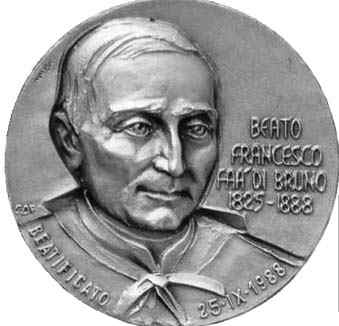
\includegraphics[width=\columnwidth]{Faa_di_Bruno_4.jpeg}
\end{column}
\end{columns}}\only<2>{
\begin{alertblock}{Faà di Bruno’s formula for RL operators}
If $f$ and $g$ are \emph{regular enough} we have\vspace{-1em}
\[ 
\begin{split}
{}_{RL}{D_{[a,t]}^{\alpha}} [fg](t) = \sum_{k=1}^{+\infty} \binom{\alpha}{k} \frac{k! (t-a)^{k-\alpha}}{\Gamma(k-\alpha+1)} \sum_{\ell=1}^{k} \left( {}_{RL}{D_{[a,t]}^{\ell}} f \right)(g(t)) \\ \sum_{(a_1,\cdots,a_k) \in A_{k,\ell}} \prod_{r=1}^{k} \frac{1}{a_r!} \left( \frac{ \frac{d^r}{d t^r} g(t) }{r} \right)^{a_r} + \frac{(t-a)^{-\alpha}}{\Gamma(1-\alpha)} f(g(t)),
\end{split}
\]
where $(a_1,\ldots,a_k) \in A_{k,\ell}$ means that\vspace{-1em}
\[
a_1,\ldots,a_k \in \mathbb{N}_0, \, \sum_{r=1}^{k} r a_r = k \text{ and } \sum_{r=1}^{k} a_r = \ell.
\]
\end{alertblock}
}

\end{frame}

\section{Towards differential equations}

\begin{frame}{What now?}
We have put together \textbf{all the analogues of the instruments of classical calculus}, but what do we do with them now?
\vfill
\onslide<2->{What we would like to solve is:
\[
{}_{RL}{D_{[0,t]}^{\alpha}} \mathbf{y}(t) = f(t,\mathbf{y}(t)), \qquad \mathbf{y}\,:\,[0,T] \rightarrow \mathbb{R}^d, \; f : [0,T] \times \mathbb{R}^d \rightarrow \mathbb{R}^d. 
\]
Nevertheless, we \alert{have a problem!} What we would like to solve is a Cauchy problem, so we need to put \textbf{initial conditions}, but last time we observed that\vspace{-1em}
\[
{}_{RL}{D_{[0,t]}^{\alpha}} \mathbf{c} \neq 0, \qquad \mathbf{c} \in \mathbb{R}^d.
\]
Therefore, we should equip the system with the \alert{\textbf{following initial conditions}} instead\vspace{-1em}
\[
{}_{RL}{D_{[0,t]}^{\alpha - k}} \mathbf{y}(0) = \mathbf{b}_k, \quad k = 1,2,\ldots,\lceil \alpha \rceil - 1, \; \lim_{z \rightarrow 0^+} I_{[0,t]}^{\lceil \alpha \rceil - \alpha} \mathbf{y}(z) = b_{\lceil \alpha \rceil}.
\]
}\onslide<3>{We could develop a theory for this, but \alert{\textbf{these conditions are physically difficult}} to use, we don't get this type of initial data from the applications.}

\end{frame}

\section{Caputo fractional derivatives}

\begin{frame}{Caputo fractional derivatives}
\begin{columns}
\begin{column}{0.7\columnwidth}
\begin{block}{Caputo fractional derivative~\parencite{CaputoOriginal}}
Let $\alpha \geq 0$, and $m = \lceil \alpha \rceil$. Then, we define the operator
\[
{}_{C}{D_{[a,t]}^{\alpha}} f = I_{[a,t]}^{m-\alpha} \frac{d^m}{d t^m} f,
\]
whenever $\frac{d^m}{d t^m} f \in \mathbb{L}^1([a,b])$.
\end{block}
\end{column}
\begin{column}{0.25\columnwidth}
\scriptsize\centering 
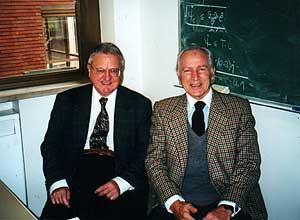
\includegraphics[width=\columnwidth]{gorcap.jpg}

(R. Gorenflo, M. Caputo, Bologna 2000, source: \href{http://www.fracalmo.org}{fracalmo.org})
\end{column}
\end{columns}
\vfill
\begin{itemize}
	\item[\faLightbulb] We have exchanged the order of the derivative and fractional integral operators.
\end{itemize}
\vfill
\onslide<2>{
\begin{quote}
	``Chi cerca trova, chi ricerca ritrova.'' - E. De Giorgi
\end{quote}
The concept occurred a certain number of times: \parencite{rabotnov1969creep,MR0224984,MR24764,MR0025899,liouville1832memoire}.
}

\end{frame}

\begin{frame}{So, what is the difference?}

First of all, we have the result we wanted on constants $c \in \mathbb{R}$:
\[
{}_{C}{D_{[a,t]}^{\alpha}} c = I_{[a,t]}^{m-\alpha} \frac{d^m}{d t^m} c = I_{[a,t]}^{m-\alpha} 0 = 0.
\]
\onslide<2>{We can put in relation the two operators with the following result}
\begin{alertblock}<2>{Theorem}
Let $\alpha > 0$ and $m = \lceil \alpha \rceil$. Moreover, assume that $f \in \mathbb{A}^m([a,b])$. Then,
\[
{}_{C}{D_{[a,t]}^{\alpha}} f = {}_{RL}{D_{[a,t]}^{\alpha}} \left[ f - T_{m-1}[f;a] \right] \text{ a.e. on }[a,b],
\]
for $T_{m-1}[f;a]$ the Taylor polynomial of degree $m-1$ for the function $f$ centered at $a$, with $T_{-1}[f;a] = 0$.
\end{alertblock}

\end{frame}

\begin{frame}{So, what is the difference?}
\textbf{Proof.} In the case $\alpha \in \mathbb{N}$ the result follows easily, since both quantities reduces to the integer order $\alpha$th derivative.\only<2->{ Therefore, we consider the case $\alpha \notin \mathbb{N}$ and $m = \lceil \alpha \rceil > \alpha$
\[
\begin{split}
{}_{RL}{D_{[a,t]}^{\alpha}} \left[ f - T_{m-1}[f;a] \right] = & \frac{d^m}{d t^m} I_{[a,t]}^{m-\alpha}  \left[ f - T_{m-1}[f;a] \right] \\
= & \alert<8>{\frac{d^m}{d t^m}} \alert<3>{\int_{a}^{t} \frac{(t-\tau)^{m-\alpha-1}}{\Gamma(m-\alpha)}\left( f(\tau) - T_{m-1}[f;a](\tau) \right)\,\textrm{d}\tau},
\end{split}
\]
}\only<3-4>{We apply a \textbf{partial integration} 
\[
\begin{split}
\alert<3>{*} = & \left. -\frac{1}{\Gamma(m-\alpha+1)} \left[ (f(\tau) - T_{m-1}[f,a](\tau))(t-\tau)^{m-\alpha} \right] \right|_{\alert<4>{\tau = a}}^{\alert<4>{\tau = t}} \\
 & + \frac{1}{\Gamma(m-\alpha+1)} \int_{a}^{t} ( f'(\tau) - (T_{m-1}[f,a](\tau))' ) (t-\tau)^{m-\alpha}\,\textrm{d}\tau.
\end{split}
\]
}\only<4>{
The \alert<4>{terms in red} are zero, and only the integral terms remain. 
}\only<5-6>{We apply a \textbf{partial integration} $m$ times since $f \in \mathbb{A}^m([a,b])$: 
\[
I_{[a,t]}^{m-\alpha} \left[ f - T_{m-1}[f;a] \right] = I_{[a,t]}^{2m - \alpha} \frac{d^m}{d t^m} \left[ f - T_{m-1}[f;a] \right] = I_{[a,t]}^{m } I_{[a,t]}^{m - \alpha} \alert<6>{\frac{d^m}{d t^m}} \left[ f - \alert<6>{T_{m-1}[f;a]} \right],
\]
}\only<7->{We apply a \textbf{partial integration} $m$ times since $f \in \mathbb{A}^m([a,b])$ and obtain the expression
\[ I_{[a,t]}^{m-\alpha} \left[ f - T_{m-1}[f;a] \right] = I_{[a,t]}^{m} I_{[a,t]}^{m - \alpha} \frac{d^m}{d t^m} f. \]}\only<6>{
the $m$th derivative of the Taylor polynomial is zero (degree $m-1$).}\only<8->{We reapply the $m$th derivative to the simplified expression: 
\[
{}_{RL}{D_{[a,t]}^{\alpha}} \left[ f - T_{m-1}[f;a] \right] = \alert<8>{\frac{d^m}{d t^m}} I_{[a,t]}^{m} I_{[a,t]}^{m - \alpha} \frac{d^m}{d t^m} f = I_{[a,t]}^{m - \alpha} \frac{d^m}{d t^m} f = {}_{C}{D_{[a,t]}^{\alpha}} f.
\]
} 
 
\end{frame}

\begin{frame}{An example of computation}
Let $f(t) = (t-a)^\beta$ for some $\beta \geq 0$, then
\[
{}_{CA}D_{[a,t]}^\alpha f(t) = \begin{cases}
0, & \beta \in \{0,1,2,\ldots,\lceil \alpha \rceil-1\},\\
\frac{\Gamma(\beta + 1)}{\Gamma(\beta +1-\alpha)} (t - a)^{\beta - \alpha}, & (\beta \in \mathbb{N}\,\land\,\beta \geq \lceil \alpha \rceil)\\
& \lor\,(\beta \notin \mathbb{N} \land \beta > \lceil \alpha \rceil - 1).
\end{cases}
\]
Let us compare it with the Riemann-Liouville case:
\[
{}_\text{RL}D_{[0,1]}^\alpha f(t) = \begin{cases}
0, & \alpha-\beta \in \mathbb{N}, \\
\frac{\Gamma(\beta + 1)}{\Gamma(\beta + 1 - \alpha)} (t-a)^{\beta - \alpha}, & \alpha - \beta \notin \mathbb{N}. \\
\end{cases}
\]
\begin{itemize}
	\item[\faExclamation] The two operators have different kernels and domain.
\end{itemize}
\end{frame}

\subsection{Properties}

\begin{frame}{Caputo fractional derivatives - Properties}
We can rewrite all the properties we have seen for RL derivatives for the Caputo version.

\begin{alertblock}{Theorem. (Caputo Derivatives Properties)}
Let $\alpha \geq 0$ and $m = \lceil \alpha \rceil$
\begin{enumerate}[(i)]
\item ${}_{C}{D_{[a,t]}^{\alpha}}f = {}_{RL}{D_{[a,t]}^{\alpha}} f - \sum_{k=0}^{m-1} \nicefrac{ f^{(k)}(a) }{\Gamma(k-\alpha+1)}(t-a)^{k-\alpha}$,  
\item ${}_{C}{D_{[a,t]}^{\alpha}}f = {}_{RL}{D_{[a,t]}^{\alpha}} f$ iff $f$ has a zero of order $m$ at $a$,
\item If $f$ is continuous, $ {}_{C}{D_{[a,t]}^{\alpha}} I_{[a,t]}^{\alpha} f = f$,
\item If $f \in \mathbb{A}^{m}([a,b])$ then $I_{[a,t]}^{\alpha} {}_{C}{D_{[a,t]}^{\alpha}} = f(t) - \sum_{k=0}^{m-1} \nicefrac{f^{(k)}(a)}{k!}(x-a)^k$,
\item If $f \in \mathcal{C}^k([a,b])$, $\alpha,\beta > 0$ s.t. $\exists \ell \in \mathbb{N}$ $\ell \leq k$ and $\alpha,\alpha+\beta \in [\ell-1,\ell]$ then ${}_{C}{D_{[a,t]}^{\alpha}}{}_{C}{D_{[a,t]}^{\beta}} f = {}_{C}{D_{[a,t]}^{\alpha+\beta}}f$.
\item $f \in \mathcal{C}^{\mu}([a,b])$, $\alpha \in [0,\mu]$, then ${}_{RL}{D_{[a,t]}^{\mu - \alpha}} {}_{C}{D_{[a,t]}^{\alpha}} f = f^{(\mu)}$.
\end{enumerate}
\end{alertblock}
\end{frame}

\begin{frame}{Caputo fractional derivatives - Properties}
\begin{alertblock}{Theorem. (Caputo Derivatives Properties)}
\begin{enumerate}[(i)]
	\setcounter{enumi}{6}
	\item For $f_1,f_2 \,:[a,b]\rightarrow \mathbb{R}$, $c_1,c_2 \in \mathbb{R}$ then
	\[
	{}_{C}{D_{[a,t]}^{\alpha}}(c_1 f_1 + c_2 f_2) = c_1 {}_{C}{D_{[a,t]}^{\alpha}}f_1 + c_2 {}_{C}{D_{[a,t]}^{\alpha}} f_2 \text{ a.e. on }[a,b], 
	\]
	if ${}_{C}{D_{[a,t]}^{\alpha}}f_1$, ${}_{C}{D_{[a,t]}^{\alpha}}f_2$ exist a.e. on $[a,b]$,
	\item \alert{(Leibniz)} let $\alpha \in (0,1)$, $f,g$ analytic on $(a-h,a+h)$, then
	\[
	\begin{split}
	{}_{C}{D_{[a,t]}^{\alpha}}[fg](t) = & \frac{(t-a)^{-\alpha}}{\Gamma(1-\alpha)}g(a)( f(t) - f(a)) + \left({}_{C}{D_{[a,t]}^{\alpha}}(g(t)\right)f(t) \\ & \qquad + \sum_{k=1}^{\infty} \binom{\alpha}{k} \left( I_{[a,t]}^{k-\alpha} g(t) \right) {}_{C}{D_{[a,t]}^{k}}f(t).
	\end{split}
	\]
\end{enumerate}
\end{alertblock}
They can all be proved by mimicking the proofs for the RL derivative.
\end{frame}



\section{Fractional ODEss with Caputo Derivatives}

\begin{frame}{Fractional ODEs with Caputo Derivatives}
Let's restart with the differential equation, but now written in terms of Caputo Derivatives
\begin{equation}\label{eq:fode}
\alpha > 0,\quad m = \lceil \alpha \rceil, \qquad \begin{cases}
\displaystyle {}_{C}{D_{[0,t]}^{\alpha}} \mathbf{y}(t) = f(t,\mathbf{y}(t)), & t \in [0,T],\\[0.5em]
\displaystyle \frac{d^k \mathbf{y}(0)}{d t^k}  = \mathbf{y}_0^{(k)}, & k=0,1,\ldots,m-1.
\end{cases}\tag{FODE}
\end{equation}

And we are now faced with the usual questions
\definecolor{success}{HTML}{4a934a}
\definecolor{todo}{HTML}{0099cc}
\begin{itemize}
\item[\only<1>{\faQuestionCircle}\only<2>{\textcolor{success}{\faQuestionCircle}}] Is there any solution? \only<2>{\textcolor{success}{ $\rightarrow$ This lecture}}
\item[\only<1>{\faQuestionCircle}\only<2>{\textcolor{success}{\faQuestionCircle}}] If there is at least one, then how many there are?\only<2>{\textcolor{success}{ $\rightarrow$ This lecture}}
\item[\only<1>{\faQuestionCircle}\only<2>{\textcolor{todo}{\faQuestionCircle}}]  When it is all said and proved, how can we approximate it?\only<2>{\textcolor{todo}{ $\rightsquigarrow$ The next one}}
\end{itemize}
\end{frame}

\begin{frame}{A Peano existence theorem for first order equations}

\begin{alertblock}{Theorem \parencite[Theorem 2.1,2.2]{DiethelmFord}}
Let $0 < \alpha$  and $m = \lceil \alpha \rceil$. Moreover let $\{ y_0^{(k)} \in \mathbb{R} \}_{k=0}^{m-1}$, $K > 0$, and $h^* > 0$. We define
\[
G = \left\lbrace (t,y) \,:\, t \in [0,h^*] \,:\, \left| y - \sum_{k=0}^{m-1} t^k \nicefrac{y_0^{(k)}}{k!} \right| \leq K  \right\rbrace,
\]
and let the function $f: G \rightarrow \mathbb{R}$ be continuous. Furthermore, define
\[
M = \sup_{(t,z) \in G} |f(t,z)|, \; h = \begin{cases}
h^*, & \text{ if }M=0,\\
\min \{ h^*, (K \nicefrac{\Gamma(\alpha+1)}{M})^{\nicefrac{1}{n}} \}, & \text{ else.}
\end{cases}
\]
Then, there exists a function $y \in \mathcal{C}([0,h])$ solving~\eqref{eq:fode}.
\end{alertblock}

\onslide<2>{To prove it we need a Lemma\ldots and a bit of work.}

\end{frame}

\begin{frame}{A Peano existence theorem for first order equations}
\begin{alertblock}{Lemma}
Under the same hypotheses of the previous Theorem. A function $y \in \mathcal{C}([0,h])$ is a solution of the
initial value problem~\eqref{eq:fode} \emph{if and only if} it is a solution of the nonlinear Volterra
integral equation of the second kind
\[
y(t) = \sum_{k=0}^{m-1} \frac{t^k}{k!} y_0^{(k)} + \frac{1}{\Gamma(\alpha)} \int_{0}^{t} (t-\tau)^{\alpha-1} f(\tau,y(\tau))\,\textrm{d}\tau, \quad m = \lceil \alpha \rceil.
\] 
\end{alertblock}

\textbf{Proof.} We need to prove both the implications.%
\only<2-3>{\textcolor{blue}{$(\Rightarrow)$} First of all we have $y(t)$ being a continuous solution of the nonlinear Volterra equation. We apply on both side the Caputo derivative of order $\alpha$ 
\only<2>{\[
{}_{C}{D_{[0,t]}^{\alpha}} y(t) = \underbrace{{}_{C}{D_{[0,t]}^{\alpha}} \left[ \sum_{k=0}^{m-1} \frac{t^k}{k!} y_0^{(k)} \right]}_{= 0\, \; \lceil \alpha \rceil > m - 1} + {}_{C}{D_{[0,t]}^{\alpha}} \left[ \int_{0}^{t} (t-\tau)^{\alpha-1} f(\tau,y(\tau))\,\textrm{d}\tau \right],
\]}\only<3>{\[
{}_{C}{D_{[0,t]}^{\alpha}} y(t) = {}_{C}{D_{[0,t]}^{\alpha}} I^{\alpha}_{[0,t]}f(t,y(t)) = f(t,y(t)),\, f \text{ is continuous}.
\]
}}\only<4->{\textcolor{blue}{$(\Rightarrow)$} follows by direct computation.}\only<4->{ \textcolor{blue}{$(\Leftarrow)$} Is a bit more laborious. Let us define $z(t) = f(t,y(t)) \in \mathcal{C}[0,h]$, we can rewrite \eqref{eq:fode} as:
\only<4>{\[
z(t) = f(t,y(t)) = {}_{C}D^\alpha_{[0,t]} y(t) = {}_{RL}D^{\alpha}_{[0,t]} ( y - T_{m-1}[y;0](t))  = \frac{d^m}{d t^m} I_0^{m-\alpha}(y - T_{m-1}[y;0])(t),
\]}
\only<5>{we have an equality between continuous function, so we can apply $I^{m}_{[0,t]}$ to both sides!}
\only<6>{
\[
I^{m}_{[0,t]} z(t) = I^{m}_{[0,t]}  \frac{d^m}{d t^m} I_0^{m-\alpha}(y - T_{m-1}[y;0])(t) = I_0^{m-\alpha}(y - T_{m-1}[y;0])(t) + q(t),
\]
for a polynomial $q(t) \in \mathbb{P}_{\leq m - 1}[t]$.
}
\only<7-8>{\vspace{-0.7em}
\begin{columns}
\begin{column}{0.3\columnwidth}
\[\begin{split}&I^{m}_{[0,t]} z(t) = \\ &I_0^{m-\alpha}(y - T_{m-1}[y;0])(t) + q(t) \end{split} \]
\end{column}
\begin{column}{0.65\columnwidth}
\only<7>{
\begin{itemize}
\item $I^{m}_{[0,t]} z(t) = 0$ (at least) $m$times for $t = 0$,
\item $y - T_{m-1}[y;0] = 0$ (at least) $m$times for $t = 0$,
\item[$\Rightarrow$] $I_0^{m-\alpha}(y - T_{m-1}[y;0])(t) = 0$ (at least) $m$times for $t = 0$,
\end{itemize}}\only<8>{Therefore $q(t) = 0$ (at least) $m$times for $t = 0$, but $\operatorname{deg}(q) \leq m-1$ $\Rightarrow$ $q \equiv 0$.}
\end{column}
\end{columns}
}
\only<9>{
\[ I^{m}_{[0,t]} z(t) = I_0^{m-\alpha}(y - T_{m-1}[y;0])(t) \]	
and apply ${}_{RL}D^{m-\alpha}_{[0,t]}$ to both side of the equation.
}
\only<10>{
\[
{}_{RL}D^{m-\alpha}_{[0,t]} I_0^{m-\alpha}(y - T_{m-1}[y;0])(t) = {}_{RL}D^{m-\alpha}_{[0,t]} I^{m}_{[0,t]} z(t) 
\]
}
\only<11>{
\[
\begin{split}
(y - T_{m-1}[y;0])(t) = &  {}_{RL}D^{m-\alpha}_{[0,t]} I^{m}_{[0,t]} z(t)  = \frac{d}{d t} I_{[0,t]}^{1+\alpha-m} I_{[0,t]}^{m} z(t) = \frac{d}{dt} I_{[0,t]}^{1+\alpha} z(t) = I_0^{\alpha} z(t).
\end{split}
\]
}
\only<12>{
\[
y(t) = \sum_{k=0}^{m-1} \frac{t^k}{k!} y_0^{(k)} + \frac{1}{\Gamma(\alpha)} \int_{0}^{t} (t-\tau)^{\alpha-1} f(\tau,y(\tau))\,\textrm{d}\tau.
\]
by recalling the definitions of $T_{m-1}[y,0]$ and the RL-integral.
}
}
\end{frame}

\begin{frame}[fragile]{A Peano existence theorem for first order equations}
The other two results we will need (and that we are not going to prove) are
\begin{alertblock}{Theorem (Ascoli-Arzelà)}
Lef $F \subset \mathcal{C}([a,b])$ for some $a < b$, and assume the sets to be equipped with the supremum norm. Then $F$ is \emph{relatively compact}\footnotemark[1] in $\mathcal{C}([a,b])$ if $F$ is \begin{itemize}
	\item \emph{uniformly bounded}, $\exists\,C > 0$ s.t. $\|f\|_{\infty} \leq C$ $\forall\,f \in F$,
	\item \emph{equicontinuous} $\forall\,\varepsilon > 0$ $\exists\,\delta > 0$ such that $\forall\,f \in F$ and all $x,x* \in [a,b]$ with $|x-x^*| < \delta$ we have $|f(x)-f(x^*)| < \varepsilon$.
\end{itemize}
\end{alertblock}

\begin{alertblock}{Schauder’s Fixed Point Theorem}
Lef $(E,d)$ be a complete metric space, let $U$ be a closed convex subset of $E$, and let $A : U \rightarrow U$ be a mapping such that the set $\{ A u \,:\; u \in U\}$ is \emph{relatively compact}\footnotemark[1]  in $E$. Then $A$ has at least one fixed point.
\end{alertblock}

\footnotetext[1]{A subset whose closure is compact.}
\end{frame}

\begin{frame}{A Peano existence theorem for first order equations}
Let us look again at the statement of the Theorem.
\begin{alertblock}{Theorem \parencite[Theorem 2.1,2.2]{DiethelmFord}}
	Let $0 < \alpha$  and $m = \lceil \alpha \rceil$. Moreover let $\{ y_0^{(k)} \in \mathbb{R} \}_{k=0}^{m-1}$, $K > 0$, and $h^* > 0$. We define
	\[
	G = \left\lbrace (t,y) \,:\, t \in [0,h^*] \,:\, \left| y - \sum_{k=0}^{m-1} t^k \nicefrac{y_0^{(k)}}{k!} \right| \leq K  \right\rbrace,
	\]
	and let the function $f: G \rightarrow \mathbb{R}$ be continuous. Furthermore, define
	\[
	M = \sup_{(t,z) \in G} |f(t,z)|, \; h = \begin{cases}
	h^*, & \text{ if }M=0,\\
	\min \{ h^*, (K \nicefrac{\Gamma(\alpha+1)}{M}^{\nicefrac{1}{n}} \}, & \text{ else.}
	\end{cases}
	\]
	Then, there exists a function $y \in \mathcal{C}([0,h])$ solving~\eqref{eq:fode}.
\end{alertblock}
\end{frame}

\begin{frame}{A Peano existence theorem for first order equations}
\textbf{Proof.} \only<1>{If $M = 0$, then $f(x,y) = 0$ for all $(x,y) \in G$, then we can explicitly write the solution as 
\[
y : [0,h] \rightarrow \mathbb{R}\, \qquad y(t) = \sum_{k=0}^{m-1} \frac{t^k}{k!} y_0^{(k)},
\]
therefore a solution exists.}\only<2-4>{If $M > 0$, let us apply the \textbf{Lemma} and rewrite our problem as a Volterra equation:
\[
y(t) = \sum_{k=0}^{m-1} \frac{t^k}{k!} y_0^{(k)} + \frac{1}{\Gamma(\alpha)} \int_{0}^{t} (t-\tau)^{\alpha-1} f(\tau,y(\tau))\,\textrm{d}\tau, \quad m = \lceil \alpha \rceil,
\]
and introduce the polynomial $T$ satisfying the boundary condition and the space $U$
\[
T(t) = \sum_{k=0}^{m-1} \frac{x^k}{k!} y_0^{(k)}, \quad U = \{ y \in \mathcal{C}([0,h]) \,:\,\|y - T\|_{\infty} \leq K \}.
\]\only<3>{
\begin{itemize}
	\item $U$ is closed and convex,
	\item $U \subset \mathcal{C}([0,h])$,
	\item[$\Rightarrow$] $U$ is a non empty Banach space (at least $T \in U$). 
\end{itemize}}
\only<4>{Let us define the operator:
\[
(A y)(t) = T(t) + \frac{1}{\Gamma(\alpha)} \int_{0}^{t} (t-\tau)^{\alpha-1} f(\tau,y(\tau))\,{\textrm d}\tau.
\]}
}\only<5>{If $M > 0$, let us apply the \textbf{Lemma} and rewrite our problem as a Volterra equation:
\[
y = A y, \quad (A y)(t) = T(t) + \frac{1}{\Gamma(\alpha)} \int_{0}^{t} (t-\tau)^{\alpha-1} f(\tau,y(\tau))\,{\textrm d}\tau.
\]
\alert{\faLightbulb} we have to prove that $A$ has a fixed point by the following steps:
\begin{enumerate}
	\item proving that $A y \in U$,
	\item showing that $A(U) = \{A u \,:\, u \in U\}$ is \emph{relatively compact} (Ascoli-Arzelà),
	\item apply Schauder's Fixed Point Theorem for the victory \faHandPeace.
\end{enumerate}
}
\only<6-12>{\emph{Step 1.} Let us take $0 \leq t_1 \leq t_2 \leq h$
\only<6-7>{
\[
\begin{split}
| (Ay)(t_1) - (Ay)(t_2) | = & \frac{1}{\Gamma(\alpha)} \left| \int_{0}^{t_1} (t_1 - \tau)^{\alpha-1} f(\tau,y(\tau))\,\textrm{d}\tau - \int_{0}^{t_2} (t_2 - \tau)^{\alpha-1} f(\tau,y(\tau))\,\textrm{d}\tau \right| \\
= &  \frac{1}{\Gamma(\alpha)} \left| \int_{0}^{t_1} \left[ (t_1 - \tau)^{\alpha-1} - (t_2 - \tau)^{\alpha-1} \right] f(\tau,y(\tau))\,\textrm{d}\tau \right. \\ & \left. - \int_{t_1}^{t_2} (t_2 - \tau)^{\alpha-1} f(\tau,y(\tau))\,\textrm{d}\tau \right| \\
\leq & \frac{M}{\Gamma(\alpha)} \left( \int_{0}^{t_1} \left| (t_1 - \tau)^{\alpha-1} - (t_2 - \tau)^{\alpha-1} \right|\,\textrm{d}\tau + \only<6>{\int_{t_1}^{t_2} (t_2 - \tau)^{\alpha-1}\,\textrm{d}\tau}\only<7->{ \frac{(t_2 - t_1)^\alpha}{\alpha} } \right)
\end{split} 
\]}
\only<8>{
\[
| (Ay)(t_1) - (Ay)(t_2) | \leq \frac{M}{\Gamma(\alpha)} \left( \alert<8>{\int_{0}^{t_1} \left| (t_1 - \tau)^{\alpha-1} - (t_2 - \tau)^{\alpha-1} \right|\,\textrm{d}\tau} +  \frac{(t_2 - t_1)^\alpha}{\alpha} \right).
\]
If $\alpha = 1$ the first integral vanishes. 

If $\alpha < 1$, $\alpha - 1 < 0$, and hence $(t_1 - \tau)^{\alpha-1} \geq (t_2 - \tau)^{\alpha-1}$, thus we remove the $|\cdot|$ and
\[
\int_{0}^{t_1} \left| (t_1 - \tau)^{\alpha-1} - (t_2 - \tau)^{\alpha-1} \right| = \frac{1}{\alpha} (t_1^\alpha - t_2^\alpha + (t_2 - t_1)^\alpha) \leq \frac{1}{\alpha} (t_2 - t_1)^\alpha.
\]

If $\alpha > 1$ we have $(t_1 - \tau)^{\alpha-1} \leq (t_2 - \tau)^{\alpha-1}$
\[
\int_{0}^{t_1} \left| (t_1 - \tau)^{\alpha-1} - (t_2 - \tau)^{\alpha-1} \right| = \frac{1}{\alpha} (t_2^\alpha - t_1^\alpha - (t_2 - t_1)^\alpha) \leq \frac{1}{\alpha} (t_2^\alpha - t_1^\alpha).
\]
}
}
\only<9-12>{
\[
| (Ay)(t_1) - (Ay)(t_2) | \leq
\begin{cases}
\nicefrac{2M}{\Gamma(\alpha + 1)}(t_2 - t_1)^\alpha, & \alpha \leq 1,\\
\nicefrac{M}{\Gamma(\alpha + 1)}( (t_2 - t_1)^\alpha + t_2^\alpha - t_1^\alpha ), & \alpha > 1.
\end{cases}
\]
Therefore,
\begin{itemize}
	\item<10-> $Ay$ is continuous since $| (Ay)(t_1) - (Ay)(t_2) | \rightarrow 0$ for $t_2 \rightarrow t_1$,
	\item<11-> for $y \in U$ and $t \in [0,h]$ we find \only<12>{$| (Ay)(t) - T(t) | \leq K$}
	\item[$\Rightarrow$]<12-> $Ay \in U$ if $y \in U$.
\end{itemize}
\only<11>{
\[
\begin{split}
| (Ay)(t) - T(t) | = & \frac{1}{\Gamma(\alpha)} \left| \int_{0}^{t} (t-\tau)^{\alpha-1} f(\tau,y(\tau)) \right| \leq \frac{1}{\Gamma(\alpha+1)} M t^\alpha \leq \frac{1}{\Gamma(\alpha+1)} M h^\alpha \\
\text{\footnotesize $\left({\text{Hp: } h < K \frac{\Gamma(\alpha+1)}{M}^{\nicefrac{1}{n}} }\right)$} \leq & \frac{1}{\Gamma(\alpha+1)} M \frac{K \Gamma(\alpha+1)}{M} = K.
\end{split}
\]
}
}%
\only<13-17>{Our plan:
\begin{enumerate}
	\setcounter{enumi}{1}
	\item[\faCheck] proving that $A y \in U$,
	\item showing that $A(U) = \{A u \,:\, u \in U\}$ is \emph{relatively compact} (Ascoli-Arzelà),
	\item apply Schauder's Fixed Point Theorem for the victory \faHandPeace.
\end{enumerate}
\emph{Step 2.} First we prove that the set is \emph{bounded}, let $z \in A(U)$ and $t \in [0,h]$
\[
\begin{split}
|z(t)| \only<13>{= |(Ay)(t)| \leq & \|T\|_{\infty} + \frac{1}{\Gamma(\alpha)} \int_{0}^{t} (t-\tau)^{\alpha-1} |f(\tau,y(\tau))|\,\textrm{d}\,\tau \\
\leq & \|T\|_{\infty} + \frac{1}{\Gamma(\alpha+1)} M h^\alpha} \leq \|T\|_\infty + K.
\end{split}
\]
\only<14>{
For the \emph{emicontinuity}, let $0 \leq t_1 \leq t_2 \leq h$ we found (for $\alpha \leq 1$)
\[
| (Ay)(t_1) - (Ay)(t_2) | \leq  \frac{2M}{\Gamma(\alpha + 1)}(t_2 - t_1)^\alpha \leq \frac{2M}{\Gamma(\alpha+1)}\delta^\alpha, \quad \text{ if } |t_2 - t_1| < \delta.
\]
the expression on the right is independent of $y$,$t_1$, and $t_2$.
}
\only<15->{
For the \emph{emicontinuity}, let $0 \leq t_1 \leq t_2 \leq h$ we found (for $\alpha > 1$)
\only<15-16>{
\[
\begin{split}
| (Ay)(t_1) - (Ay)(t_2) | \leq & \frac{M}{\Gamma(\alpha + 1)}( (t_2 - t_1)^\alpha + t_2^\alpha - t_1^\alpha ), \only<15>{\\ 
\text{\footnotesize (Mean Value Theorem) } = & \frac{M}{\Gamma(\alpha+1)} ( (t_2 - t_1)^\alpha + \alpha(t_2 - t_1)\tau^{\alpha - 1} ), \quad \tau \in [t_1,t_2] \subseteq [0,h]} \\
\only<16>{ \leq & \frac{M}{\Gamma(\alpha+1)} ( (t_2 - t_1)^\alpha + \alpha(t_2 - t_1)h^{\alpha - 1} ) }  
\end{split}
\]
}%
\only<17>{
\[
| (Ay)(t_1) - (Ay)(t_2) | \leq \frac{M}{\Gamma(\alpha + 1)} (\delta^\alpha + \alpha \delta h^\alpha - 1), \quad \text{ if } |t_2 - t_1 | < \delta,
\]
the expression on the right is again independent of $y$,$t_1$, and $t_2$.
}
}%
}%
\only<18->{Our plan:
\begin{enumerate}
	\setcounter{enumi}{2}
	\item[\faCheck] proving that $A y \in U$,
	\item[\faCheck] showing that $A(U) = \{A u \,:\, u \in U\}$ is \emph{relatively compact} (Ascoli-Arzelà),
	\only<18>{\item apply Schauder's Fixed Point Theorem for the victory \faHandPeace.}
	\only<19>{\item[\faCheck] apply Schauder's Fixed Point Theorem for the victory \faHandPeace.}
\end{enumerate}

Finally we have all the ingredients:
\begin{itemize}
	\item $E = \mathcal{C}([0,h])$, $U = \{ y \in \mathcal{C}([0,h]) \,:\,\|y - T\|_{\infty} \leq K \}$ is a closed, convex subset of $E$.
	\item We have proved that the operator $A$ is such that $\{ Au \,:u\in U \}$ is relatively compact in~$E$.
	\item[$\Rightarrow$] By \alert{Schauder's Fixed Point Theorem} we have the existence of \emph{at least} a solution. \hfill \qedsymbol
\end{itemize}
}
\begin{onlyenv}<19>
\begin{block}{At last\ldots}
We have proved existence: what about uniqueness?
\end{block}
\begin{exampleblock}{\faCode\,A programming idea}
We could use the fixed-point iteration as an algorithm for obtaining a solution.
\end{exampleblock}
\end{onlyenv}
\end{frame}

\begin{frame}{Uniqueness of the solution à-la-Picard-Lindel\"of}
As for the classical calculus case, to prove \emph{uniqueness} we need Lipschitzianity of the system dynamics w.r.t. to the second component.

\begin{alertblock}<2->{Weissinger’s Fixed Point Theorem}
Assume $(U,d)$ to be a nonempty complete metric space, and let $\beta_j \geq 0$ for every $j \in \mathbb{N}_0$ and such that $\sum_{j=0}^{\infty} \beta_j$ converges. Furthermore, let the mapping $A\,:\,U \rightarrow U$ satisfy the inequality
\[
d(A^j u, A^j v) \leq \beta_j d(u,v), \quad \forall j \in \mathbb{N}, \quad \forall\,u,v \in U.
\]
Then $A$ has a \emph{uniquely determined fixed point} $u^*$. Moreover, for any $u_0 \in U$, the sequence $(A^j u_0)_{j=1}^{\infty}$ converge to this fixed point.
\end{alertblock}
\onslide<3>{The plan}
\begin{itemize}
	\item[\faRecycle]<3> Reuse the same set $U$, and map $A$ from the existence proof,
	\item[\faLessThanEqual]<3> Prove the inequality and give an expression of the $\alpha_j$ in term of the Lipschitz constant.
\end{itemize}

\end{frame}

\begin{frame}{Uniqueness of the solution à-la-Picard-Lindel\"of}
\begin{alertblock}{Theorem}\small
Let $0 < \alpha$ and $m = \lceil \alpha \rceil$. Moreover, let $y_0^{(0)},\ldots,y_0^{(m-1)} \in \mathbb{R}$, $K > 0$, and $h^* > 0$. We define the same set $G$:\vspace{-0.3em}
\[
G = \left\lbrace (t,y) \,:\, t \in [0,h^*] \,:\, \left| y - \sum_{k=0}^{m-1} t^k \nicefrac{y_0^{(k)}}{k!} \right| \leq K  \right\rbrace,
\]
and let the function $f : G \rightarrow \mathbb{R}$ be continuous and Lipschitz w.r.t. the second entry\vspace{-0.3em}
\[
|f(t,y_1) - f(t,y_2)| \leq L |y_1 - y_2|,
\]
for some $L > 0$ independently of $t,y_1$, and $y_2$. Then, for $h$ such that\vspace{-0.3em}
\[
M = \sup_{(t,z) \in G} |f(t,z)|, \; h = \begin{cases}
h^*, & \text{ if }M=0,\\
\min \{ h^*, (K \nicefrac{\Gamma(\alpha+1)}{M}^{\nicefrac{1}{n}} \}, & \text{ else.}
\end{cases}
\]
there exist a uniquely defined $y \in \mathcal{C}[0,h]$ solving \eqref{eq:fode}.
\end{alertblock}
\end{frame}

\begin{frame}{Uniqueness of the solution à-la-Picard-Lindel\"of}
\textbf{Proof.} We are under the same hypotheses of the \textbf{Existence Theorem}, thus \eqref{eq:fode} has a solution.

We prove\only<10->{d} \textbf{by induction} on $j$ that
\[
\| A^j y - A^j \tilde{y} \|_{\infty} \leq \frac{(L t^\alpha)^j}{\Gamma(1+\alpha j)} \|y - \tilde{y} \|_\infty \only<10>{ = \alpha_j \|y - \tilde{y}\|_\infty, \qquad \alpha_j = \frac{(Lh)^\alpha}{\Gamma(1+\alpha j)}}.
\]
\only<2>{\emph{Base case:} $j = 0$ follows by the definition.}%
\only<3-9>{\noindent\emph{Inductive hypothesis:} we assume it true for $j-1$ and prove it for $j$.

\emph{Inductive step:} 
\[
\begin{split}
\| A^j y - A^j \tilde{y} \|_{\infty} \only<1-8>{= & \| A(A^j-1 y) - A(A^{j-1}\tilde{y})\|_{\infty} \\}
\only<3>{= & \frac{1}{\Gamma(\alpha)} \sup_{0 \leq w \leq t} \left| \int_{0}^{w} (w-\tau)^{\alpha-1} \left[ f(\tau,A^{j-1}y(\tau)) - f(\tau,A^{j-1}\tilde{y}(\tau)) \right]\,\textrm{d}\tau \right| \\}
\only<3-4>{\text{\small(Lipschitz) }\leq & \frac{L}{\Gamma(\alpha)}  \sup_{0 \leq w \leq t}  \int_{0}^{w} (w-\tau)^{\alpha-1} \left| A^{j-1}y(\tau) - A^{j-1}\tilde{y}(\tau) \right|\,\textrm{d}\tau \\}
\only<4-5>{ \leq & \frac{L}{\Gamma(\alpha)}  \int_{0}^{w} (w-\tau)^{\alpha-1} \sup_{0 \leq w \leq \tau}  \left| A^{j-1}y(w) - A^{j-1}\tilde{y}(w) \right|\,\textrm{d}\tau \\}
\only<5-6>{ \text{\small (I.H.) } \leq & \frac{L^j}{\Gamma(\alpha)\Gamma(1+\alpha(j-1))} \int_{0}^t (t-\tau)^{\alpha -1} t^{\alpha(j-1)} \sup_{0 \leq w \leq \tau} | y(w)- \tilde{y}(w)|\,\textrm{d}\tau \\}
\only<6-7>{ \leq & \frac{L^j}{\Gamma(\alpha)\Gamma(1+\alpha(j-1))}  \sup_{0 \leq w \leq t} | y(w)- \tilde{y}(w)| \int_{0}^t (t-\tau)^{\alpha -1} t^{\alpha(j-1)}\,\textrm{d}\tau \\}
\only<7-8>{ \leq & \frac{L^j}{\Gamma(\alpha)\Gamma(1+\alpha(j-1))}  \| y - \tilde{y}\|_\infty \frac{\Gamma(\alpha)\Gamma(1+\alpha(j-1))}{\Gamma(1+\alpha j)} t^{\alpha j}
}
\only<9>{ \leq \frac{(L t^\alpha)^j}{\Gamma(1+\alpha j)} \|y - \tilde{y} \|_\infty. }
\end{split} 
\]
}
\only<10->{
To apply Weissinger’s Fixed Point Theorem we need to prove that the series $\displaystyle \sum_{j=0}^{+\infty} \alpha_j = \sum_{j=0}^{+\infty}\frac{(Lh)^\alpha}{\Gamma(1+\alpha j)}$ converges.
\begin{exampleblock}{Mittag-Leffler}
\[
E_\alpha(z) = \sum_{k=0}^{+\infty} \frac{z^\alpha}{\Gamma(\alpha k + 1)}, \quad \alpha > 0 \qquad \text{ is an entire function.}
\]
\end{exampleblock}
}

\end{frame}

\begin{frame}{State of the art}
We have proved that the \emph{Cauchy problem}
\[
\alpha > 0,\quad m = \lceil \alpha \rceil, \qquad \begin{cases}
\displaystyle {}_{C}{D_{[0,t]}^{\alpha}} \mathbf{y}(t) = f(t,\mathbf{y}(t)), & t \in [0,T],\\[0.5em]
\displaystyle \frac{d^k \mathbf{y}(0)}{d t^k}  = \mathbf{y}_0^{(k)}, & k=0,1,\ldots,m-1.
\end{cases}
\]
admits
\begin{itemize}
	\item for $f$ continuous a \emph{local} solution in $\mathcal{C}([0,h])$, $h < h^*$,
	\item for $f$ continuous and Lipschitz in the second entry a \emph{local} and \emph{unique} solution in $\mathcal{C}([0,h])$, $h < h^*$.
\end{itemize}
\onslide<2>{For \alert{classical ODEs} this is the point in which one starts proving \emph{extension results} for the solutions. They exist also for the Fractional case. We are going to state them without proof.}
\end{frame}

\begin{frame}{Extension results}

\begin{exampleblock}{Corollary}
Assume the hypotheses of the existence Theorem, but substitute $G$ with the domain of definition of $f$, i.e., $G = [0,h^*] \times \mathbb{R}$. Moreover, assume that $f$ is continuous and that there exist constants $c_1 \geq 0$,$c_2 \geq 0$, $0 \leq \mu < 1$ such that
\[
f(t,y) \leq c_1 + c_2 |y|^\mu, \quad \forall\,(t,y) \in G.
\]
Then, there exists a function $y \in \mathcal{C}([0,h^*])$ solving \eqref{eq:fode}.
\end{exampleblock}
	\begin{itemize}
		\item Since $G$ is no longer compact we need to demand a suitable bound explicitly, Weierstrasse Theorem no longer applies,
		\item A sufficient condition on $f$ to imply the decay we need is for $f$ to be continuous and bounded on $G$,
		\item[{\alert{\faExclamationTriangle}}] Our condition is violated already by linear equations!
	\end{itemize}

\end{frame}

\begin{frame}{Extension results}

\begin{alertblock}{Theorem}
Let $0 < \alpha$ and $m = \lceil \alpha \rceil$. Moreover, let $y_0^{(0)},\ldots,y_0^{(m-1)} \in \mathbb{R}$ and $h^* > 0$. We define the set $G = [0,h^*] \times \mathbb{R}$ and let $f\,:G \rightarrow \mathbb{R}$ be continuous and fulfill a Lipschitz condition with respect to the second variable with a Lipischitz constant $L$ that is independent of $t$, $y_1$, and $y_2$. Then there exist a uniquely defined function $y \in \mathcal{C}([0,h^*])$ solving the \eqref{eq:fode}.
\end{alertblock}

\begin{itemize}
	\item[\faBook] For a \textbf{proof} see the proof of Theorem 6.8 from \parencite[pp 96-102]{DiethelmBook} that is inspired by the proof for Volterra integral equations in~\parencite[Theorem 4.8]{MR796318}.
	\item[{\faSmile[regular]}] We can now solve \alert{linear equations} 
	\[
	{}_{CA}D_{[0,t]}^\alpha y(t) = f(t)y(t) + g(t), \qquad f,g \in \mathcal{C}([0,h^*]), \quad L = \|f\|_{\infty} < \infty.
	\]
	\item<2>[\faQuestionCircle] Do we know hot to solve by hand any simple FODE? 
\end{itemize}

\end{frame}

\subsection{Simple cases and representation formulas}

\begin{frame}{Simple cases and representation formulas}
The simplest ODE we know ho to solve is the \emph{relaxation equation}
\[
\mathbb{R} \ni \lambda < 0, \quad \begin{cases}
y'(t) = \lambda y(t), & t \in [0,T],\\
y(0) = y_0,
\end{cases} \qquad y(t) = y_0 \exp(\lambda t).
\]
\begin{exampleblock}<2->{Relaxation FODE}
Let $\alpha > 0$, $m = \lceil \alpha \rceil$ and $\lambda \in \mathbb{R}$. The solution of the Cauchy problem
\[ {}_{CA}D_{[0,t]}y(t) = \lambda y(t), \quad y(0) = y_0, \quad y^{(k)}(0) = 0, \quad k=1,2,\ldots,m-1, \]
is given by
\[
y(t) = y_0 E_\alpha(\lambda t^\alpha), \quad t \geq 0.
\]
\end{exampleblock}
\begin{itemize}
	\item<3> The previous existence result tells us that the problem has indeed a \emph{unique solution}.
\end{itemize}
\end{frame}

\begin{frame}{Solution of the relaxation FODE}
\begin{exampleblock}{Two parameters Mittag-Leffler}
	\[
	E_{\alpha,\beta}(z) = \sum_{k=0}^{+\infty} \frac{z^\alpha}{\Gamma(\alpha k + \beta)}, \quad \alpha,\beta > 0 \qquad \text{ is an entire function.}
	\]
\end{exampleblock}

To see that this is the case we can use \textbf{Stirling formula} and \textbf{root test}
\begin{description}
	\item[Stirling:] $\Gamma(x+1) = \left(\nicefrac{x}{e}\right)^x \sqrt{2\pi x}(1 + o(1))$ for $x \rightarrow +\infty$,
	\item[Root test:] $\sum_{n=1}^{+\infty} a_n$ converge absolutely if $C = \limsup_{n \rightarrow + \infty} \sqrt[n]{|a_n|} < 1$.
\end{description}
We write
\[
a_j^{\nicefrac{1}{j}} = \left( \frac{e}{j\alpha + \beta} \right)^{ \nicefrac{\alpha+\beta}{j} } (2\pi(\alpha j + \beta))^{-\nicefrac{1}{2j}} (1+o(1)) \rightarrow 0 \text{ for } j \rightarrow \infty.
\]
Thus the \alert{radius of convergence} is infinite.
\end{frame}

\begin{frame}{Solution of the relaxation FODE}
\[ \alpha > 0, \; m = \lceil \alpha \rceil, \; {}_{CA}D_{[0,t]}y(t) = \lambda y(t), \quad y(0) = y_0, \quad y^{(k)}(0) = 0, \quad k=1,2,\ldots,m-1, \]
\only<1-2>{
\begin{enumerate}
	\item<1-> $y(0) = y_0 E_{\alpha}(0) = y_0$ since
	\[
	E_\alpha(z) = 1 + \frac{z}{\Gamma(\alpha + 1)} + \frac{z^2}{\Gamma(2\alpha + 1)} + \ldots,
	\]
	\item<2-> If $\alpha > 1$, $m \geq 2$, $y^{(k)}(0) = 0, \quad k=1,2,\ldots,m-1$
	\[
	y(t) = 1 + \frac{\lambda t^\alpha}{\Gamma(\alpha+1)} + \frac{\lambda^2 t^{2\alpha} }{\Gamma(2\alpha+1)} + \ldots,
	\]
	imposing the condition on the derivatives implies 
	\[
	y^{(k)}(t) = \frac{\lambda t^{\alpha-k}}{\Gamma(\alpha+1-k)} + \frac{\lambda^2 t^{2\alpha - k} }{\Gamma(2\alpha+1-k)} + \ldots, \quad k=1,2,\ldots,m-1.
	\]
\end{enumerate}}
\only<3->{Let $p_k(t) = t^k$
\begin{equation*}
\begin{split}
\alert<10>{{}_{CA}D_{[0,t]}y(t) =} & \; {}_{CA}D_{[0,t]} \left[ \sum_{j=0}^{+\infty} \frac{(\lambda p_\alpha)^j}{\Gamma(j\alpha+1)} \right] = I_{0}^{m-\alpha} \frac{d^m}{d t^m} \left[  \sum_{j=0}^{+\infty} \frac{\lambda^j p_{j\alpha} }{\Gamma(j\alpha+1)} \right] \onslide<4->{ \\
= & I_{0}^{m-\alpha} \left[  \sum_{j=\alert<4>{1}}^{+\infty} \frac{ \frac{d^m}{d t^m} \lambda^j p_{j\alpha} }{\Gamma(j\alpha+1)} \right]
} \onslide<5->{ = I_{0}^{m-\alpha} \left[  \sum_{j=1}^{+\infty} \frac{ \lambda^j p_{j\alpha \alert<5>{- m} } }{\Gamma(j\alpha+1\alert<5>{-m} )} \right] }\only<6-8>{ \\
= & \sum_{j=1}^{+\infty} \frac{ \lambda^j \alert<6>{I_{0}^{m-\alpha}} p_{j\alpha -m } }{\Gamma(j\alpha+1 -m  )} 
} \only<7>{
= \sum_{j=1}^{+\infty} \frac{ \lambda^j  p_{j\alpha - \alpha } }{\Gamma(j\alpha+1 - \alpha  )} 
} \only<8->{
\only<9->{\\}= \only<9->{&} \sum_{j=1}^{+\infty} \frac{ \lambda^j  t^{j\alpha - \alpha } }{\Gamma(j\alpha+1 - \alpha  )} 
} \only<9>{
\sum_{j=\alert<9>{0}}^{+\infty} \frac{\lambda^{j\alert<9>{+1}} t^{\alpha j}}{\Gamma(\alpha j + 1)}
}\only<10>{
= \alert<10>{\lambda y(t)}.
}
\end{split}
\end{equation*}
}

\end{frame}

\begin{frame}{Why only continuous solutions?}
The existence theorems we have seen give us a solution $y(t) \in \mathcal{C}([0,h])$, can we have more?

\begin{block}<2->{Regularity for ODEs}
\[k \in \mathbb{N}, \; f \in \mathcal{C}^{k-1}([y_0 - K, y_0 + k]\times \mathbb{R}), \; \begin{cases} y'(t) = f(t,y(t)),\\y(0) = y_0 \end{cases} \; \Rightarrow \; y(t) \in \mathcal{C}^k.\]
\end{block}

\onslide<3>{We can reuse our \alert{example computation}:

\[f(t) = (t-a)^\beta, \; \frac{\Gamma(\beta + 1)}{\Gamma(\beta +1-\alpha)} (t - a)^{\beta - \alpha}, \; \beta \notin \mathbb{N} \land \beta > \lceil \alpha \rceil - 1  \]

If we select $a = 0$, $\alpha = \nicefrac{1}{2}$, $\beta = \nicefrac{1}{2}$, then
\[
\begin{cases}
{}_{CA}D_{[0,t]}y(t) = \Gamma(\nicefrac{3}{2}),\\
y(0) = 0,
\end{cases} \, \Rightarrow \, y(t) = \sqrt{x}.
\] 
From an \alert{analytic right-hand side} we got a \alert{non differentiable solution}.
}
\end{frame}

\begin{frame}{Why only continuous solutions?}

\begin{block}{\faLuggageCart\;Take-home message}
Regularity of the right-hand side of the \eqref{eq:fode} is \alert{not sufficient} to ensure regularity of the solution.
\end{block}

\begin{itemize}
	\item[{\faFile[regular]}] Some more restrictive conditions under which regularity can be ensured can be found in \parencite{DiethelmRegularity}, to give an idea, one have to further ensure conditions for the zeros of $z(t) = f(t,y(t))$.
	\item Furthermore, if the solution of \eqref{eq:fode} is analytic, but not a polynomial of degree $\lceil \alpha \rceil - 1$, then $f$ is not analytic.
	\item<2> This will be important when we try do design \emph{numerical methods}, since many results on convergence order usually rely on the regularity of the solution. Going high-order in the fractional settings is not in general an easy task!
\end{itemize}

\end{frame}

\subsection{The Mittag-Leffler Function}

\begin{frame}{The Mittag-Leffler Function}
The $E_{\alpha,\beta}(z)$ takes the role of the exponential function when moving from ODEs to FODEs.
\[
E_{\alpha,\beta}(z) = \sum_{k=0}^{+\infty} \frac{z^\alpha}{\Gamma(\alpha k + \beta)}, \quad \alpha,\beta > 0.
\]
\begin{itemize}
	\item[\faQuestionCircle] How can we compute it?
	\begin{itemize}
		\item<2->[\faDoorClosed] Using the series representation,
		\item<3->[\faDoorClosed] A quadrature formula applied to an integral representation,
		\item<4->[\only<4>{\faDoorClosed}\only<5>{\faDoorOpen}] Inversion of the Laplace transform.
	\end{itemize}
\end{itemize}
\begin{block}<5>{Laplace Transform}
For a real- or complex-valued function $f(t)$ of the real variable $t$ defined on $\mathbb{R}$ the (two-sided) Laplace transform is defined as
\[
F(s) = \mathcal{L}\{f\}(s) = \int_{-\infty}^{+\infty} e^{-st} f(t)\,\textrm{d}t.
\]
\end{block}
\end{frame}

\begin{frame}[fragile]{Inverting the Laplace Transform}
If we want fo compute $f(t)$ and have access to $F(s) = \mathcal{L}\{f\}(s)$ we can perform a \emph{numerical inversion}, that is
\begin{columns}
\begin{column}{0.6\columnwidth}
\[
f(t) = \frac{1}{2 \pi i} \int_{\sigma - i \infty}^{\sigma + \infty} e^{st} F(s)\,\textrm{d}s.
\]
where 
\begin{itemize}
	\item $(\sigma - i \infty,\sigma + i \infty)$ is called the \alert{Bromwich line},
	\item $\sigma$ is such that all the \textcolor{blue}{singularities} of $F(s)$ lies to the left $\Re{(s)} = \sigma$.
\end{itemize}
\begin{exampleblock}{\faExclamationTriangle\;Branch lines}
If $F(s)$ is a \emph{multivalued function} we need to add a branch-cut to make the integrand single-valued.
\end{exampleblock}
\end{column}
\begin{column}{0.4\columnwidth}
\begin{tikzpicture}
\begin{axis}[
width=\columnwidth,
height=\columnwidth,
axis x line=center,
axis y line=center,
xlabel={$\Re(z)$},
ylabel={$\Im(z)$},
xticklabels={,,},
yticklabels={,,},
xlabel style={below right},
ylabel style={above left},
xmin=-5,
xmax=5,
ymin=-5,
ymax=5]
\addplot[thick, samples=50, smooth,domain=0:6,red] coordinates {(2,-5)(2,5)};
\addplot[mark=*] coordinates {(2,0)} node[pin=-20:{$\sigma$}]{} ;
\addplot[mark=x,blue] coordinates {(1,1)};
\addplot[mark=x,blue] coordinates {(1,-1)};
\end{axis}
\end{tikzpicture}
\end{column}
\end{columns}


\end{frame}

\begin{frame}[fragile]{Inverting the Laplace Transform}

To numerically approximate the integral 
\[
f(t) = \frac{1}{2 \pi i} \int_{\sigma - i \infty}^{\sigma + i \infty} e^{st} F(s)\,\textrm{d}s.
\]
we \textbf{always need a change of variable}, the exponential term \emph{oscillates wildly} and \emph{decays slowly} along the Bromwich line. 

We have to \alert{change the countour of integration} to something more suitable, i.e., we change
\[
s = s(u) \,\mapsto\, f(t) = \frac{1}{2\pi i} \int_{-\infty}^{+\infty} e^{s(u)t} F(s(u))s'(u)\,\textrm{d}u,
\]
and then approximate the integral with the \emph{trapezoidal rule} with spacing $h$
\[
f_{h,N}(t) = \frac{h}{2\pi i} \sum_{k=-N}^{N} e^{s(u_k)t} F(s(u_k)) s'(u_k), \quad u_k = kh. 
\]
\end{frame}

\begin{frame}[fragile]{Inverting the Laplace Transform}

\faQuestionCircle\, What is the \textbf{best contour}?
\begin{columns}
\begin{column}{0.6\columnwidth}
\begin{itemize}
	\item<2-> Parabolic contour:
		\[
		s = \mu (i u + 1)^2, \qquad - \infty < u < \infty 
		\]
	\item<3-> Hyperbolic contour:
		\[
		s = \mu (1 + \sin(i u - \alpha)), \qquad - \infty < u < \infty 
		\]	
	\item<4-> Talbot contour:
		\[
		s = -\sigma + \mu \theta \cot(\alpha \theta) + i \theta \nu,  \qquad - \pi \leq \theta \leq \pi
		\]
\end{itemize}
\end{column}
\begin{column}{0.4\columnwidth}
\begin{onlyenv}<2>
\begin{tikzpicture}
\begin{axis}[
width=\columnwidth,
height=\columnwidth,
axis x line=center,
axis y line=center,
xlabel={$\Re(z)$},
ylabel={$\Im(z)$},
xticklabels={,,},
yticklabels={,,},
xlabel style={below right},
ylabel style={above left},
xmin=-5,
xmax=5,
ymin=-5,
ymax=5]
\addplot[red,domain=-10:10] plot[smooth]({-0.25*x^2+2},{x});
\addplot[mark=*] coordinates {(2,0)} node[pin=-20:{$\sigma$}]{} ;
\addplot[mark=x,blue] coordinates {(1,1)};
\addplot[mark=x,blue] coordinates {(1,-1)};
\end{axis}
\end{tikzpicture}
\end{onlyenv}%
\begin{onlyenv}<3>
\begin{tikzpicture}
\begin{axis}[
width=\columnwidth,
height=\columnwidth,
axis x line=center,
axis y line=center,
xlabel={$\Re(z)$},
ylabel={$\Im(z)$},
xticklabels={,,},
yticklabels={,,},
xlabel style={below right},
ylabel style={above left},
xmin=-5,
xmax=5,
ymin=-5,
ymax=5]
\addplot[red,domain=-10:10] plot[smooth]({ 0.25*(14 - 3*sqrt(4 + \x*\x))},{x});
\addplot[mark=*] coordinates {(2,0)} node[pin=-20:{$\sigma$}]{} ;
\addplot[mark=x,blue] coordinates {(1,1)};
\addplot[mark=x,blue] coordinates {(1,-1)};
\end{axis}
\end{tikzpicture}
\end{onlyenv}%
\begin{onlyenv}<4->
\begin{tikzpicture}
\begin{axis}[
trig format plots=rad,
width=\columnwidth,
height=\columnwidth,
axis x line=center,
axis y line=center,
xlabel={$\Re(z)$},
ylabel={$\Im(z)$},
xticklabels={,,},
yticklabels={,,},
xlabel style={below right},
ylabel style={above left},
xmin=-5,
xmax=5,
ymin=-5,
ymax=5]
\addplot [domain=-3.01:3.01,red] plot[smooth]({1 + x*cot(x)}, {x});
\addplot[mark=*] coordinates {(2,0)} node[pin=-20:{$\sigma$}]{} ;
\addplot[mark=x,blue] coordinates {(1,1)};
\addplot[mark=x,blue] coordinates {(1,-1)};
\end{axis}
\end{tikzpicture}
\end{onlyenv}
\end{column}
\end{columns}

\onslide<5>{Selecting \textbf{contour} and \textbf{parameters} depends on the \textbf{error analysis}.}

\end{frame}

\begin{frame}[fragile]{Inverting the Laplace Transform}

\begin{itemize}
	\item[\faBrain] All the contours exploit the fact that $e^{st}$ decays rapidly as $\Re(s) \rightarrow - \infty$,
	\item \textbf{Trapezoidal rule} for integral on the real line for which the integrand decay sufficiently rapidly is \textbf{exponential}:
	\only<1>{\begin{alertblock}{Theorem \parencite[Theorem 5.1]{Trapezoidal}}\small
	Suppose that $w$ is analytic in the strip $|\Im(x)| < a$ for some $a > 0$. Suppose further that $w(x) \rightarrow 0$ uniformly as $|x| \rightarrow + \infty$ in the strip, and that for some $M$ it satisfies\vspace{-0.5em}
	\[
	\int_{-\infty}^{+\infty} |w(x+ib)|\,\textrm{d}x \leq M, \quad \forall b \in (-a,a),
	\]
	then for any $h > 0$, the trapezoidal rule $w_{h,N}$ with step-size $h$ exists and satisfies\vspace{-0.5em}
	\[
	|w_h - \int_{-\infty}^{+\infty}w(x)\,\textrm{d}x | \leq \frac{2 M}{\exp(\nicefrac{2\pi a}{h}) - 1},
	\]
	and the quantity $2M$ on the numerator is as small as possible.
	\end{alertblock}}
\end{itemize}

\begin{onlyenv}<2>
\begin{exampleblock}{Steepest descent contours}
For some functions it is possible to use a technique called ``saddle point technique'' from complex analysis to estimate the asymptotic of complex integrals. This determines the optimal steepest descent contour.
\end{exampleblock}


References for the general problem are:
\begin{description}
	\item[Talbot:] \cite{Dingfelder,Weideman1,Schmelzer},
	\item[Parabolic \& Hyperbolic:] \cite{WeidemanTrefethen}.
\end{description}
\end{onlyenv}

\end{frame}

\begin{frame}{Our case: we've got poles and a branch cut}
In our case the function for which we can compute the \emph{Laplace transform} is
\[
e_{\alpha,\beta}(t;\lambda) = t^{\beta - 1} E_{\alpha,\beta}(t^\alpha \lambda), \quad t \in \mathbb{R}_+, \qquad \lambda \in \mathcal{C}.
\]
That is given by
\[
\mathcal{E}_{\alpha,\beta}(t;\lambda) = \frac{s^{\alpha-\beta}}{s^\alpha - \lambda}, \quad \Re(s) > 0, \qquad |\lambda s^{-\alpha}| < 1.
\]
\begin{itemize}
	\item<2-> There are non-integer powers $\Rightarrow$ $\mathcal{E}_{\alpha,\beta}$ is a \alert{multivalued function} and a branch-cut on the real negative semi-axis is needed,
	\item<3-> We have also the \textbf{poles} for $\theta = \arg(\lambda)$
	\[ \overline{s}^*_j = \lambda^{\nicefrac{1}{\alpha}} = | \lambda |^{\nicefrac{1}{\alpha}} e^{i\frac{\theta + 2\pi j}{\alpha}}, \quad \left\lbrace j \in \mathbb{Z} \,\left| - \frac{\alpha}{2} - \frac{\theta}{2\pi} < j \leq \frac{\alpha}{2} - \frac{\theta}{2\pi} \right. \right\rbrace, \] 
\end{itemize}
\onslide<4>{
\alert{\faExclamationTriangle}\,There could be lots of poles! Finding suitable contours is difficult. 
}
\end{frame}

\begin{frame}[fragile]{Cauchy’s residue theorem to the rescue}
We can use Cauchy’s residue theorem if we have too many poles
\[
e_{\alpha,\beta}(t;\lambda) = \sum_{s^* \in \mathcal{S}^*_\mathcal{C}} \operatorname{Res}(e^{st} \mathcal{E}_{\alpha,\beta}(s;\lambda), s^*) + \frac{1}{2\pi i} \int_{\mathcal{C}} e^{st} \mathcal{E}_{\alpha,\beta}(s;\lambda)\,\textrm{d}s.
\]
\begin{columns}
\begin{column}{0.6\columnwidth}
\begin{itemize}
	\item $\mathcal{S}^*_\mathcal{C}$ is the set of all singularities lying on the rightmost part of the complex plane delimited by~$\mathcal{C}$,
	\item We can compute the residual in close form:
	\[
	\operatorname{Res}(e^{st} \mathcal{E}_{\alpha,\beta}(s;\lambda), s^*) = \frac{1}{\alpha} (s^*)^{1-\beta} e^{s^* t}.
	\]
\end{itemize}
\end{column}
\begin{column}{0.4\columnwidth}
	\begin{tikzpicture}
	\begin{axis}[
	width=0.8\columnwidth,
	height=0.8\columnwidth,
	axis x line=center,
	axis y line=center,
	xlabel={$\Re(z)$},
	ylabel={$\Im(z)$},
	xticklabels={,,},
	yticklabels={,,},
	xlabel style={below right},
	ylabel style={above left},
	xmin=-5,
	xmax=5,
	ymin=-5,
	ymax=5]
	\addplot[red,domain=-10:10] plot[smooth]({-0.25*x^2+2},{x});
	\addplot[mark=*] coordinates {(2,0)} node[pin=-20:{$\sigma$}]{} ;
	\addplot[mark=x,blue] coordinates {(0,0)};
	\addplot[mark=x,blue] coordinates {(1,1)};
	\addplot[mark=x,blue] coordinates {(-0.5,-1)};
	\addplot[mark=x,blue] coordinates {(-3,2)};
	\addplot[mark=x,blue] coordinates {(-4,-2)};
	\addplot[mark=x,cyan] coordinates {(-1,-4)};
	\addplot[mark=x,cyan] coordinates {(3,+4)};
	\end{axis}
	\end{tikzpicture}
\end{column}
\end{columns}
\end{frame}

\begin{frame}{The full algorithm \parencite{Garrappa}}

To build the full algorithm few technical steps are needed:
\begin{enumerate}
	\item<1-> Finding an ordering of the poles,
	\[
	\phi(s) = \frac{\Re(s) + |s|}{2}, \qquad 0 = \phi(s_0^*) < \phi(s_1^*) < \cdots < \phi(s_J^*), 
	\]
	\item<2-> Consider $J+1$ parabolas $s = \phi(s^*_j) (u + 1)^2$ and the relevant $J+1$ plane regions $R_j$,
	\item<3-> The regions $R_j$ are the analyticity regions to use in the Trefethen and Weideman result,
	\item<4-> Obtain bounds on the discretization error and use it to determine optimal $\mu_j$, step-size $h_j$ and number of quadrature nodes $N_k$,
	\item<5-> Select the best region $R_j$ w.r.t. the lowest computation and reduction of round-off errors.
\end{enumerate}

\onslide<6>{\faCode\, \href{https://it.mathworks.com/matlabcentral/fileexchange/48154-the-mittag-leffler-function}{it.mathworks.com/matlabcentral/fileexchange/48154-the-mittag-leffler-function}}

\end{frame}

\begin{frame}{Summary and anticipations}
\definecolor{success}{HTML}{4a934a}
\definecolor{todo}{HTML}{0099cc}

We did
\begin{itemize}
	\item[\textcolor{success}{\faCheckCircle}] Uncovered properties of Riemann-Liouville Derivatives,
	\item[\textcolor{success}{\faCheckCircle}] Introduced the Caputo Derivative,
	\item[\textcolor{success}{\faCheckCircle}] Formulation, existence and uniqueness results for FODEs,
	\item[\textcolor{success}{\faCheckCircle}] The Mittag-Leffler function and its computation.
\end{itemize}
Next up
\begin{itemize}
	\item[\textcolor{todo}{\faClipboardList}] Numerical methods for the integration of FODEs.
\end{itemize}
\end{frame}

\appendix

\section*{Bibliography}
{\unnumbered
\begin{frame}[allowframebreaks,noframenumbering]{Bibliography}
\small
\printbibliography

\end{frame}
}
\end{document}

